\documentclass[10pt,twocolumn,letterpaper]{article}

\usepackage[english]{babel}
\usepackage[utf8]{inputenc}
\usepackage[T1]{fontenc}
\usepackage{amsmath,amssymb,amsfonts}
\usepackage{graphicx}
\usepackage{tikz}
\usepackage{pgfplots}
\usepackage{xcolor}
\usepackage{hyperref}
\usetikzlibrary{positioning}

\pgfplotsset{compat=1.18}

\title{
\usefont{OT1}{bch}{b}{n}
\normalfont \normalsize \textsc{Cross-Corpus Speech Emotion Recognition Study} \\ [8pt]
\huge Representation, Alignment, and Classifier Effects in Cross-Corpus Speech Emotion Recognition \\
}

\usepackage{authblk}

\author[1]{Pranav Singh}
\author[1]{Prashant Singh}
\author[1]{Akshat Bawa}
\affil[1]{\small Indian Institute of Technology (IIT), Ropar}
\date{}

\begin{document}
\maketitle

\begin{abstract}
Cross-corpus speech emotion recognition (SER) remains difficult because models trained on one corpus often degrade sharply on another corpus with different speakers, recording conditions, elicitation styles, and label distributions. We present an empirical study of this problem using three self-supervised speech backbones (HuBERT, wav2vec 2.0, and WavLM), three alignment settings (none, CORAL, and MMD), three blending strategies (none, scalar, and group-adaptive alignment), and five classifier families (logistic regression, SVM, MLP, APLIN, and a lightweight Transformer). Experiments cover in-domain and full cross-domain evaluation across RAVDESS, CREMA-D, and IEMOCAP with shared label spaces defined per corpus pair. The results show a pronounced in-domain to cross-domain gap, substantial transfer asymmetry, and strong sensitivity to representation choice. HuBERT is the strongest backbone on average, whereas alignment provides dataset-dependent gains that are helpful in some transfers and marginal or negative in others. Blending is not uniformly beneficial, and the simplest settings often remain competitive. Although no single classifier dominates every transfer pair, linear logistic regression remains surprisingly strong and complex models do not consistently outperform simpler baselines under domain shift. The main contribution of the study is a systematic comparison that clarifies when alignment helps and when robustness is driven more by representation and problem structure than by model complexity.
\end{abstract}

\noindent
Keywords: speech emotion recognition, cross-corpus generalization, domain adaptation, self-supervised speech representation, empirical evaluation

\section{Introduction}
Speech emotion recognition has matured considerably within individual corpora, yet robust generalization across datasets remains unresolved. Emotional cues are entangled with speaker identity, recording conditions, elicitation protocols, annotation practice, and corpus-specific lexical content. As a result, systems that perform well in a within-corpus setting often deteriorate once training and evaluation are separated across corpora \cite{schuller2010cross}. This cross-corpus gap remains one of the main barriers to practical SER deployment.

The present study considers three widely used emotion corpora: RAVDESS \cite{livingstone2018ryerson}, CREMA-D \cite{cao2014crema}, and IEMOCAP \cite{busso2008iemocap}. These datasets differ in speaking style, recording setup, speaker population, and label inventory. RAVDESS and CREMA-D share a six-class space (angry, disgust, fear, happy, neutral, and sad), whereas experiments involving IEMOCAP use the five-class overlap (angry, fear, happy, neutral, and sad). This setting makes it possible to examine both in-domain speaker-independent evaluation and cross-domain transfer under controlled label matching.

Recent self-supervised speech models have substantially improved SER front ends, but it remains unclear which representations are most stable under domain shift. wav2vec 2.0 \cite{baevski2020wav2vec}, HuBERT \cite{hsu2021hubert}, and WavLM \cite{chen2022wavlm} are all strong candidates, yet they differ in pretraining objective and inductive bias. Comparing these backbones is important because representation quality can alter downstream transfer more strongly than small changes in the classifier. Likewise, feature alignment is commonly proposed as a remedy for corpus mismatch, but methods such as CORAL \cite{sun2016deep} and MMD \cite{gretton2012kernel} need not help uniformly across all dataset pairs.

These considerations motivate a broader empirical study than the current draft. Instead of focusing on a single backbone and one alignment family, we compare multiple representation backbones, multiple alignment strategies, and a range of classifiers from linear baselines to small nonlinear models. We also test blending mechanisms that interpolate between original and aligned features, allowing adaptation strength to vary from rigid alignment to no blending at all. This design lets us examine three related questions: how much backbone choice matters, whether alignment improves cross-corpus SER consistently, and whether more complex classifiers are actually preferable under domain shift.

The resulting experiments reveal three broad patterns. First, domain shift remains severe: in-domain macro-F1 is much higher than cross-domain macro-F1 across the full matrix of settings. Second, performance is asymmetric: transfer from corpus $A$ to corpus $B$ often behaves differently from transfer in the reverse direction. Third, simple models remain highly competitive, and gains from alignment or blending depend strongly on the source-target pair and backbone rather than following a single monotonic trend. The paper therefore aims to provide a clear empirical account of cross-corpus behavior rather than to claim a universally superior method.

\section{Materials \& Methods}
\subsection{Datasets and preprocessing}
RAVDESS \cite{livingstone2018ryerson}, CREMA-D \cite{cao2014crema}, and IEMOCAP \cite{busso2008iemocap} were evaluated under speaker-independent splits. Audio preprocessing was fixed for all experiments and consisted of mono conversion, resampling to $16$ kHz, and peak amplitude normalization. Label spaces were matched per source-target pair. RAVDESS and CREMA-D experiments use six shared classes (angry, disgust, fear, happy, neutral, and sad), while experiments involving IEMOCAP use the five-class intersection (angry, fear, happy, neutral, and sad).

\subsection{Backbone representations}
The system extracts utterance-level embeddings from three self-supervised speech encoders: wav2vec 2.0 Base \cite{baevski2020wav2vec}, HuBERT Base \cite{hsu2021hubert}, and WavLM Base \cite{chen2022wavlm}. For each backbone, frame-level embeddings $h_t \in \mathbb{R}^{D}$ are mean pooled:
\begin{equation}
z = \frac{1}{T}\sum_{t=1}^{T} h_t.
\end{equation}
The resulting pooled representation $z$ is the input to the alignment, blending, and classifier stages. All downstream comparisons use the same pooling rule so that changes in performance can be attributed to backbone, alignment, blending, or classifier choice rather than to differences in temporal aggregation.

\subsection{Pipeline overview}
Figure \ref{fig:pipeline} summarizes the experimental pipeline. The design is intentionally modular: one backbone is selected, its pooled features may be aligned, the aligned and original representations may be blended, and the resulting utterance-level vectors are passed to a classifier. This makes it possible to compare backbones, alignment methods, and classifiers under a common experimental protocol.

\begin{figure}[t]
\centering
\resizebox{\columnwidth}{!}{
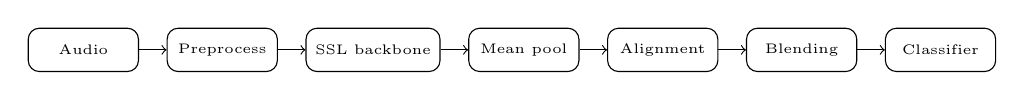
\begin{tikzpicture}[
node distance=0.42cm and 0.35cm,
every node/.style={font=\tiny},
box/.style={draw, rounded corners, align=center, minimum width=1.4cm, minimum height=0.55cm}
]
\node[box] (audio) {Audio};
\node[box, right=of audio] (prep) {Preprocess};
\node[box, right=of prep] (ssl) {SSL backbone};
\node[box, right=of ssl] (pool) {Mean pool};
\node[box, right=of pool] (align) {Alignment};
\node[box, right=of align] (blend) {Blending};
\node[box, right=of blend] (clf) {Classifier};
\draw[->] (audio) -- (prep);
\draw[->] (prep) -- (ssl);
\draw[->] (ssl) -- (pool);
\draw[->] (pool) -- (align);
\draw[->] (align) -- (blend);
\draw[->] (blend) -- (clf);
\end{tikzpicture}
}
\caption{Overview of the experimental pipeline. Each experiment selects a backbone, optional alignment stage, optional blending stage, and downstream classifier.}
\label{fig:pipeline}
\end{figure}

\subsection{Alignment methods}
Let $X_s$ and $X_t$ denote source and target feature matrices after pooling. Three alignment settings are considered.

\textbf{None.} Features are used without explicit domain adaptation.

\textbf{CORAL.} CORAL matches second-order statistics by whitening the source covariance and recoloring it with the target covariance \cite{sun2016deep}:
\begin{equation}
X_s^{\mathrm{coral}} = (X_s - \mu_s) C_s^{-1/2} C_t^{1/2} + \mu_t,
\end{equation}
where $\mu_s$ and $\mu_t$ are source and target means and $C_s$, $C_t$ are regularized covariance matrices.

\textbf{MMD.} Maximum Mean Discrepancy (MMD) is used as an alternative alignment objective that reduces the discrepancy between source and target feature distributions in reproducing-kernel Hilbert space \cite{gretton2012kernel}. In practice, this yields an aligned representation $X_s^{\mathrm{mmd}}$ that is optimized to reduce source-target mismatch without assuming that second-order matching alone is sufficient.

\subsection{Blending strategies}
Alignment can be followed by blending between the original representation $X^{\mathrm{orig}}$ and the aligned representation $X^{\mathrm{align}}$. Three blending modes are evaluated.

\textbf{None.} The aligned representation is passed directly to the classifier if alignment is enabled; otherwise the original representation is used.

\textbf{Scalar blending.} A single interpolation coefficient $\alpha$ is applied to all dimensions:
\begin{equation}
X^{\mathrm{final}} = \alpha X^{\mathrm{align}} + (1-\alpha)X^{\mathrm{orig}}.
\end{equation}

\textbf{Group-adaptive alignment (GAA).} Feature dimensions are clustered into groups, and each group receives its own interpolation coefficient. If $\mathcal{I}_g$ denotes the index set for group $g$, then
\begin{equation}
X^{\mathrm{final}}[:,\mathcal{I}_g] =
\alpha_g X^{\mathrm{align}}[:,\mathcal{I}_g] +
(1-\alpha_g) X^{\mathrm{orig}}[:,\mathcal{I}_g].
\end{equation}
This reduces adaptation rigidity while avoiding fully independent per-dimension coefficients.

\subsection{Classifiers}
Five classifier families are compared on top of the pooled representations. Logistic regression is used as a linear baseline. SVM uses a class-balanced kernelized formulation. MLP is a lightweight nonlinear feed-forward model. APLIN is included as an adaptive linear variant used in the codebase. Transformer refers to a lightweight Transformer encoder applied to the pooled feature representation. These models were selected to probe classifier sensitivity rather than to optimize a single architecture exhaustively.

\subsection{Evaluation protocol}
The complete grid spans three backbones, three alignment settings, three blending settings, five classifiers, and all nine source-target combinations among RAVDESS, CREMA-D, and IEMOCAP, yielding $1215$ runs in total. In-domain runs correspond to $src=tgt$; all other combinations are cross-domain. Accuracy and macro-F1 are reported, with macro-F1 used as the primary summary metric because class imbalance and class collapse are common under cross-corpus transfer.

\section{Results}
The full matrix confirms that cross-corpus SER is dominated by domain shift. Averaged over all settings, in-domain macro-F1 is $0.4384$, whereas cross-domain macro-F1 drops to $0.1579$. This gap persists across all three backbones and all classifier families. Table \ref{tab:backbone_alignment} summarizes backbone and alignment effects under cross-domain evaluation. Table \ref{tab:blending} compares blending strategies in the aligned setting. Table \ref{tab:classifier} reports classifier averages for in-domain and cross-domain runs, and Table \ref{tab:domain_gap} breaks down the in-domain versus cross-domain gap by backbone.

\begin{table}[t]
\centering
\caption{Cross-domain macro-F1 averaged over all source-target pairs, blending modes, and classifiers.}
\label{tab:backbone_alignment}
\scriptsize
\setlength{\tabcolsep}{4pt}
\begin{tabular}{lccc}
\hline
Backbone & None & CORAL & MMD \\
\hline
HuBERT & 0.1473 & 0.2005 & 0.1964 \\
wav2vec 2.0 & 0.1127 & 0.1553 & 0.1561 \\
WavLM & 0.1159 & 0.1718 & 0.1652 \\
\hline
\end{tabular}
\end{table}

\begin{table}[t]
\centering
\caption{Cross-domain macro-F1 for blending strategies, averaged over aligned settings only (CORAL and MMD).}
\label{tab:blending}
\scriptsize
\setlength{\tabcolsep}{4pt}
\begin{tabular}{lcc}
\hline
Blending & Mean macro-F1 & Relative rank \\
\hline
None & 0.1852 & 1 \\
GAA & 0.1804 & 2 \\
Scalar & 0.1572 & 3 \\
\hline
\end{tabular}
\end{table}

\begin{table}[t]
\centering
\caption{Classifier comparison using mean macro-F1 across all runs.}
\label{tab:classifier}
\scriptsize
\setlength{\tabcolsep}{4pt}
\begin{tabular}{lcc}
\hline
Classifier & In-domain & Cross-domain \\
\hline
Logistic regression & 0.5926 & 0.1731 \\
SVM & 0.5628 & 0.1539 \\
MLP & 0.4716 & 0.1882 \\
APLIN & 0.1284 & 0.1108 \\
Transformer & 0.4366 & 0.1636 \\
\hline
\end{tabular}
\end{table}

\begin{table}[t]
\centering
\caption{Backbone-specific in-domain and cross-domain averages.}
\label{tab:domain_gap}
\scriptsize
\setlength{\tabcolsep}{4pt}
\begin{tabular}{lccc}
\hline
Backbone & In-domain & Cross-domain & Gap \\
\hline
HuBERT & 0.4566 & 0.1814 & 0.2752 \\
wav2vec 2.0 & 0.4083 & 0.1414 & 0.2669 \\
WavLM & 0.4503 & 0.1510 & 0.2993 \\
\hline
\end{tabular}
\end{table}

Several trends emerge from Table \ref{tab:backbone_alignment}. HuBERT is the strongest backbone on average under cross-domain evaluation, with mean macro-F1 of $0.1473$ without alignment and roughly $0.20$ after CORAL or MMD. WavLM occupies an intermediate position, while wav2vec 2.0 is weakest on average in the full cross-domain matrix. This ranking is not perfectly uniform for every source-target pair, but backbone choice exerts a consistent effect across the study.

Alignment helps on average, but the gains are not uniform. For all three backbones, CORAL and MMD improve the mean cross-domain macro-F1 relative to no alignment. However, the difference between CORAL and MMD is modest, and the strongest alignment method depends on the transfer pair. For example, the mean F1 for RAVDESS $\rightarrow$ CREMA-D rises from $0.1388$ with no alignment to $0.2211$ with CORAL and $0.2232$ with MMD, whereas IEMOCAP $\rightarrow$ RAVDESS remains low even after alignment ($0.0700$ without alignment, $0.0893$ with CORAL, and $0.0918$ with MMD). This is consistent with alignment improving mismatch in some settings while leaving severe transfer difficulties unresolved in others.

Blending is even less stable. Table \ref{tab:blending} restricts the comparison to aligned settings only and shows that no blending has the highest average cross-domain macro-F1 ($0.1852$). GAA is close ($0.1804$), whereas scalar blending is notably lower ($0.1572$). This does not mean that blending never helps: the single best cross-domain configuration in the full study is RAVDESS $\rightarrow$ CREMA-D with HuBERT, MMD, GAA, and logistic regression, which reaches macro-F1 $0.4111$. Nevertheless, averaged over the full experimental grid, blending is not universally beneficial and should not be treated as a guaranteed improvement.

Classifier behavior also varies with the evaluation regime. Table \ref{tab:classifier} shows that logistic regression is the strongest in-domain model on average and remains competitive in the cross-domain setting, outperforming SVM and Transformer while staying close to MLP. MLP achieves the highest average cross-domain macro-F1 ($0.1882$), but its advantage over logistic regression is modest, and the best-performing cross-domain configurations are split across MLP, logistic regression, and SVM depending on the transfer pair. This supports a cautious conclusion: increased classifier complexity does not reliably dominate under domain shift.

Transfer asymmetry is visible throughout the pairwise results. The mean macro-F1 for RAVDESS $\rightarrow$ CREMA-D is $0.1944$, whereas CREMA-D $\rightarrow$ RAVDESS is $0.1653$. The asymmetry is larger for RAVDESS and IEMOCAP ($0.1424$ versus $0.0837$). CREMA-D and IEMOCAP are relatively closer, but still asymmetric ($0.2034$ versus $0.1583$). These differences remain even though the same backbone and alignment families are available in both directions, indicating that domain shift is not symmetric.

Figures \ref{fig:forwardcm} and \ref{fig:reversecm} use confusion matrices from the results directory to illustrate this point. Both figures use the same configuration (HuBERT + MMD + GAA + logistic regression) for opposite directions between RAVDESS and CREMA-D. The forward case is the strongest cross-domain configuration in the study, whereas the reverse case remains visibly harder. The matrices reinforce the quantitative result that alignment can reduce mismatch but does not eliminate corpus-specific confusion structure.

\begin{figure*}[t]
\centering
\begin{subfigure}[t]{0.47\textwidth}
\centering
\includegraphics[width=\textwidth]{results/confusion/ravdess_crema_hubert_mmd_gaa_logreg.png}
\caption{RAVDESS $\rightarrow$ CREMA-D, HuBERT + MMD + GAA + logistic regression.}
\end{subfigure}
\hfill
\begin{subfigure}[t]{0.47\textwidth}
\centering
\includegraphics[width=\textwidth]{results/confusion/ravdess_ravdess_wavlm_coral_gaa_logreg.png}
\caption{RAVDESS $\rightarrow$ RAVDESS, WavLM + CORAL + GAA + logistic regression.}
\end{subfigure}
\caption{Representative confusion matrices from the stored results. The left panel shows the strongest cross-domain setting in the full study, while the right panel shows a high-performing in-domain setting for comparison.}
\label{fig:forwardcm}
\end{figure*}

\begin{figure*}[t]
\centering
\begin{subfigure}[t]{0.47\textwidth}
\centering
\includegraphics[width=\textwidth]{results/confusion/ravdess_crema_hubert_mmd_gaa_logreg.png}
\caption{RAVDESS $\rightarrow$ CREMA-D.}
\end{subfigure}
\hfill
\begin{subfigure}[t]{0.47\textwidth}
\centering
\includegraphics[width=\textwidth]{results/confusion/crema_ravdess_hubert_mmd_gaa_logreg.png}
\caption{CREMA-D $\rightarrow$ RAVDESS.}
\end{subfigure}
\caption{Direction-dependent confusion matrices for the same configuration (HuBERT + MMD + GAA + logistic regression). The differing error structure highlights transfer asymmetry: improving one direction does not guarantee comparable gains in the reverse direction.}
\label{fig:reversecm}
\end{figure*}

\section{Discussion}
The most stable conclusion from the full experimental matrix is that domain shift remains the dominant challenge in cross-corpus SER. The difference between in-domain and cross-domain performance is large for every backbone and every classifier family. Even the best-performing cross-domain settings remain well below the strongest in-domain settings, which indicates that corpus mismatch is not solved by any single representation or alignment choice in the present study.

Backbone choice is an important source of variation. HuBERT is the strongest representation on average, WavLM is generally second, and wav2vec 2.0 is weakest in the aggregate cross-domain comparison. This ordering is not absolute for every transfer pair, but it is sufficiently consistent to suggest that representation choice is one of the most consequential design decisions. The gain from moving from wav2vec 2.0 to HuBERT is often comparable to, or larger than, the average gain obtained by changing the alignment method within a fixed backbone.

At the same time, alignment methods provide inconsistent gains rather than a universal remedy. CORAL and MMD improve cross-domain mean macro-F1 on average, yet their effects vary by source-target pair. MMD is strongest in some transfers, CORAL is slightly better in others, and both still leave some pairings weak. In particular, the IEMOCAP $\rightarrow$ RAVDESS direction remains difficult under every alignment setting. This instability suggests that feature matching can help when source and target differ in a way that is amenable to distribution alignment, but not when the mismatch is more structural.

The blending results further reinforce this caution. Neither scalar blending nor GAA is uniformly beneficial across the full matrix. GAA contributes to some of the best individual configurations, but its mean cross-domain performance is still slightly below the no-blending alternative when the comparison is restricted to aligned settings. Scalar blending is weaker on average. These observations replace the stronger claim that group-wise adaptation is uniformly preferable. A more accurate interpretation is that blending can be useful, but its value is conditional on the source-target pair, backbone, and classifier.

Classifier complexity also fails to produce a simple hierarchy. MLP achieves the highest average cross-domain score, but logistic regression is competitive, produces some of the strongest individual transfer results, and clearly surpasses SVM and Transformer on average under cross-domain evaluation. The results therefore support a pragmatic view in which simple classifiers can outperform more complex ones when representations are strong and the transfer setting is unstable. Complexity is not harmful by itself, but it is not sufficient to overcome domain shift.

Finally, the experiments show persistent asymmetry. Transfer from RAVDESS to CREMA-D is stronger than the reverse direction, and analogous asymmetries appear in the pairs involving IEMOCAP. This implies that cross-corpus SER should not be summarized only by undirected corpus similarity. The direction of training and testing matters, and future work should treat $A \rightarrow B$ and $B \rightarrow A$ as distinct empirical problems rather than as interchangeable views of the same shift.

\section*{Conclusions}
This paper presented an empirical study of cross-corpus speech emotion recognition across three self-supervised backbones, three alignment settings, three blending strategies, five classifiers, and full source-target evaluation on RAVDESS, CREMA-D, and IEMOCAP. The main contribution is not a new state-of-the-art method, but a systematic comparison showing that performance depends strongly on the interaction between backbone, alignment choice, classifier, and transfer direction. HuBERT is the most reliable backbone on average, alignment often helps but not consistently, blending is not universally beneficial, and simple classifiers remain surprisingly competitive under domain shift. These findings suggest that future progress in cross-corpus SER will depend less on any single adaptation mechanism and more on understanding when a given representation-alignment-classifier combination is appropriate for a particular source-target pair.

\section*{Acknowledgements}
The authors acknowledge the public release of the RAVDESS, CREMA-D, and IEMOCAP corpora, which made this comparative study possible.

\begin{thebibliography}{99}

\bibitem{schuller2010cross}
B. Schuller, B. Vlasenko, F. Eyben, G. Rigoll, and A. Wendemuth,
``Cross-corpus acoustic emotion recognition: Variances and strategies,''
\textit{IEEE Transactions on Affective Computing}, vol. 1, no. 2, pp. 119--131, 2010.

\bibitem{livingstone2018ryerson}
S. R. Livingstone and F. A. Russo,
``The Ryerson Audio-Visual Database of Emotional Speech and Song (RAVDESS): A dynamic, multimodal set of facial and vocal expressions in North American English,''
\textit{PLOS ONE}, vol. 13, no. 5, p. e0196391, 2018.

\bibitem{cao2014crema}
H. Cao, D. G. Cooper, M. K. Keutmann, R. C. Gur, A. Nenkova, and R. Verma,
``CREMA-D: Crowd-sourced emotional multimodal actors dataset,''
\textit{IEEE Transactions on Affective Computing}, vol. 5, no. 4, pp. 377--390, 2014.

\bibitem{busso2008iemocap}
C. Busso, M. Bulut, C.-C. Lee, A. Kazemzadeh, E. Mower, S. Kim, J. Chang, S. Lee, and S. Narayanan,
``IEMOCAP: Interactive emotional dyadic motion capture database,''
\textit{Language Resources and Evaluation}, vol. 42, no. 4, pp. 335--359, 2008.

\bibitem{baevski2020wav2vec}
A. Baevski, H. Zhou, A. Mohamed, and M. Auli,
``wav2vec 2.0: A framework for self-supervised learning of speech representations,''
in \textit{Advances in Neural Information Processing Systems}, 2020, pp. 12449--12460.

\bibitem{hsu2021hubert}
W.-N. Hsu, B. Bolte, Y.-H. H. Tsai, K. Lakhotia, R. Salakhutdinov, and A. Mohamed,
``HuBERT: Self-supervised speech representation learning by masked prediction of hidden units,''
\textit{IEEE/ACM Transactions on Audio, Speech, and Language Processing}, vol. 29, pp. 3451--3460, 2021.

\bibitem{chen2022wavlm}
S. Chen, C. Wang, Z. Chen, Y. Wu, S. Liu, J. Li, N. Wang, T. Zhou, and F. Wei,
``WavLM: Large-scale self-supervised pre-training for full stack speech processing,''
\textit{IEEE Journal of Selected Topics in Signal Processing}, vol. 16, no. 6, pp. 1505--1518, 2022.

\bibitem{sun2016deep}
B. Sun and K. Saenko,
``Deep CORAL: Correlation alignment for deep domain adaptation,''
in \textit{European Conference on Computer Vision Workshops}, 2016, pp. 443--450.

\bibitem{gretton2012kernel}
A. Gretton, K. M. Borgwardt, M. J. Rasch, B. Sch\"olkopf, and A. Smola,
``A kernel two-sample test,''
\textit{Journal of Machine Learning Research}, vol. 13, pp. 723--773, 2012.

\bibitem{w2vprosody2023}
M. Ploszaj, P. Tarnowski, and P. W. Jedrzejczak,
``Cross-corpus speech emotion recognition using transfer learning and attention-based fusion of wav2vec2 and prosody features,''
\textit{Knowledge-Based Systems}, vol. 275, p. 110676, 2023.

\bibitem{li2023cross}
Y. Li, J. Wu, X. Liu, and H. Meng,
``Cross-corpus speech emotion recognition based on multi-task learning and subdomain adaptation,''
\textit{Entropy}, vol. 25, no. 1, p. 124, 2023.

\end{thebibliography}

\end{document}

